\documentclass[10pt,a4paper]{article}
\usepackage[latin1]{inputenc}
\usepackage{amsmath}
\usepackage{amsfonts}
\usepackage{amssymb}
\usepackage[]{theorem}
\usepackage[nottoc]{tocbibind}
\usepackage[hidelinks]{hyperref}
\usepackage{appendix}
\usepackage{listings}
%\usepackage{minitoc}
\usepackage{graphicx}
\usepackage{float}
\usepackage{makecell}
%\usepackage{longtable}
\usepackage{textcomp}
\usepackage{authblk}
\usepackage[bottom]{footmisc}


\setlength{\topmargin}{-.5in}
\setlength{\textheight}{9in}
\setlength{\oddsidemargin}{.125in}
\setlength{\textwidth}{6.25in}

\newcommand {\subsubsubsection} [1] {\vskip 0.5em {\bf \em #1}}

%\newcommand {\comm} [1] {}
\newcommand {\comm} [1]
{
\par
\setlength{\leftskip}{-0.8in}
\begin{tabular} {p{0.1cm} | p{\textwidth}}
  {\bf ?} & {#1}
\end{tabular}
\par
\setlength{\leftskip}{0in}
}


\newcommand {\cond} {, & \textrm{if }}
\newcommand {\otherwise} {, & \textrm{else}}

\newcommand {\Forall} {\forall \ }
\newcommand {\eqdef} {\triangleq}
\newcommand {\equivalent} {\Leftrightarrow}
\renewcommand {\implies} {\Rightarrow}
\renewcommand {\impliedby} {\Leftarrow}
\renewcommand {\And}  {\ \& \ }
\newcommand {\Or}  {\ \vee \ }
\newcommand {\QED} {$\square$ \ \par }
\newcommand {\proofword}  {{\par \sf Proof:\ }}
\newcommand {\proof} [1] {\proofword #1 \QED \par}
\newcommand {\definition} [2] {\bigskip {\bf Definition} {\rm \sc #1} \par #2 \QED \bigskip}
\newcommand {\example} [2] {\bigskip {\bf Example.} {#1} \par #2 \QED}
\newcommand {\theorem} [2] {\bigskip {\bf Theorem} {\rm \sc #1} \par #2 \QED \bigskip}
\newcommand {\ve} {\mathbf}
\newcommand {\vecc} {\boldsymbol}
\newcommand {\Questions} {\vspace{5mm} {\bf Unresolved Questions:}}
\newcommand {\assert} {\square \ }

\renewcommand {\P} {\mathrm P}
\newcommand {\E} {\mathrm E \ }
\newcommand {\var} {\mathrm {var} \ }
\newcommand {\cov} {\mathrm {cov} }
\newcommand {\cor} {\mathrm {cor} }
\newcommand {\N} {\mathbb N}
\newcommand {\Z} {\mathrm Z}
\newcommand {\R} {\mathbb R}
\newcommand {\C} {\mathbb C}
\newcommand {\I} {\mathbb I}
\newcommand {\supp} {\mathrm {Supp}}
\newcommand {\mat} {\mathrm}
\newcommand {\trc} {\mathrm {tr} \ }
\newcommand {\VC} {\mathrm {VC} }
\newcommand {\const} {\mathrm {const} }
\newcommand {\sgn} {\mathrm {sgn} }
\newcommand {\dom} {\mathrm {dom} }
\newcommand {\range} {\mathrm {range} }
\newcommand {\Arg} {\mathrm {Arg} \ }

\newcommand {\LCA} {\mathrm {LCA} }  % least common ancestor (in a tree)

\newcommand {\nul} {\mathrm {null}}
\newcommand {\Dt} {\Delta t}
\newcommand {\PC} {\mathrm {PC} }
\newcommand {\MDS} {\mathrm {MDS} }
\newcommand {\CC} {\mathrm {CC} }

\newcommand {\re} {\mathrm {re}}
\newcommand {\cl} {\mathrm {cl}}
\newcommand {\intr} {\mathrm {int}}

\newcommand {\<} {\langle}
\renewcommand {\>} {\rangle}

\newcommand {\dotve} [1] {\dot {\ve #1}}

\newcommand {\la} [1] {\lambda (#1) \ }

\newcommand {\lhs} {\mathrm {lhs}}
\newcommand {\rhs} {\mathrm {rhs}}

\providecommand{\keywords}[1]
{
  \small
  \textbf{\textit{Keywords---}} #1
}

\makeatletter
\DeclareRobustCommand{\cev}[1]{%
  {\mathpalette\do@cev{#1}}%
}
\newcommand{\do@cev}[2]{%
  \vbox{\offinterlineskip
    \sbox\z@{$\m@th#1 x$}%
    \ialign{##\cr
      \hidewidth\reflectbox{$\m@th#1\vec{}\mkern4mu$}\hidewidth\cr
      \noalign{\kern-\ht\z@}
      $\m@th#1#2$\cr
    }%
  }%
}
\makeatother




\newcommand {\diff} {\Delta}


\title{Epistemic Principle of a Congruence Maximization of a Phylogenetic Tree to External Classifications
  %Taxonomy Miscongruence of Phylogenetic Trees
}
\author[1]{Slava Brover\footnote{E-mail: brovervv@ncbi.nlm.nih.gov}}
\affil[1]{\small National Center for Biotechnology Information, National Library of Medicine, National Institutes of Health, Bethesda, MD 20894, USA.}




\begin{document}
\maketitle

\begin{abstract}
A miscongruence of a phylogenetic tree to external classifications is proposed as a criterion of the quality of a phylogenetic tree.
Since an established classification of biological objects is taxonomy, 
the computation of taxonomy miscongruence between a phylogenetic tree and a given taxonomy is described.
The miscongruence with the NCBI taxonomy can be used as one number evaluating the quality of a phylogenetic tree.
The computation of taxonomy miscongruence also can be used to assign taxonomy names to interior nodes of a tree.
Taxonomy miscongruence is applied to 
comparing different phylogenetic trees, 
optimization of the parameters of a tree building,
finding taxonomically misassigned type strains,
and the analysis of the MLST clades of {\it Escherichia coli}.
\end{abstract}

\keywords {Phylogenetic tree, Tree congruence, Taxonomy, Taxonomy miscongruence, Type strain, {\it Escherichia coli}.}

%\dominitoc
\tableofcontents



\section {Introduction}

The problem of a phylogenetic tree reconstruction has a curse of lacking training sets
because there are no observed phylogenetic trees,
and yet there is a desire to reconstruct a most probable phylogenetic tree.
As a possible solution the principle of maximum congruence estimation is proposed.

This principle needs an external tree or classification and a function of miscongruence.
If a phylogenetic tree spans a large number of taxa, 
the taxonomy can be used as the reference tree
and a taxonomy miscongruence function is described.

This way a single number, miscongruence, is assigned to a phylogenetic tree,
which allows 
optimizing tree building parameters,
comparing phylogenetic trees by quality
or finding outlier objects.


\section{Methods}

\subsection {Principle of maximum congruence estimation}
\label{sec:maxCongr}

This section describes the concept and properties of miscongruence in an informal way.

Consider a set of objects 
for which it is desired to build a phylogenetic tree
and for which there exist external classifications.
For example, an external tree is a set of external classifications.

Let phylogenetic trees on these objects 
and classifications of these objects 
be represented as vectors.
Let vector~$\ve t$ be the vector representing an unknown true tree~$T$,
$\ve r$ be the vector representing external classifications~$R$,
and $\ve x$ be the vector representing an arbitrary tree~$X$,
then
\begin{equation} \label{eq:congrDeriv}
 |\ve x - \ve r|^2 = |(\ve x - \ve t) - (\ve r - \ve t)|^2 
   = |\ve x - \ve t|^2 + |\ve r - \ve t|^2 - 2 (\ve x - \ve t)^t (\ve r - \ve t).
\end{equation}
If the deviations of~$\ve x$ and~$\ve r$ from~$\ve t$ are independent,
then on the average $(\ve x - \ve t)^t (\ve r - \ve t) = 0$,
and 
$$ \arg \min_{\ve x} |\ve x - \ve r|^2 = \arg \min_{\ve x} |\ve x - \ve t|^2 $$
which is generalized as
\begin{equation*}
 \arg \min_{\theta \in \Theta} \diff (X(\theta),R) = \arg \min_{\theta \in \Theta} \diff(X(\theta),T),
\end{equation*}
where 
$X(\theta)$ is the tree built with parameters $\theta \in \Theta$,
and $\diff(T_1,T_2)$ is a {\em miscongruence} between trees or classifications~$T_1$ and~$T_2$.

Minimizing the miscongruence of the tree~$X(\theta)$ from external classifications~$R$ by selecting parameters~$\theta \in \Theta$,
in other words, maximizing the congruence between~$X(\theta)$ and~$R$,
on the average minimizes the miscongruence of~$X(\theta)$ from the true tree~$T$.

Therefore, building a phylogenetic tree of high quality consists in 
selecting~$\Theta$ and~$R$
and computing 
$$ \arg \min_{\theta \in \Theta} \diff (X(\theta),R). $$

The miscongruence consists of the two parts:
$$ \diff (X(\theta),R) = \diff_0 + \diff_1, $$
where 
\begin{itemize}
  \item $\diff_0$ matches $|\ve x - \ve t|^2$ in~(\ref{eq:congrDeriv}), which is minimized with the minimization of the miscongruence;
  \item $\diff_1$ matches $ |\ve r - \ve t|^2 - 2 (\ve x - \ve t)^t (\ve r - \ve t)$ in~(\ref{eq:congrDeriv}),
       which is noise and creates a lower bound of the miscongruence.
\end{itemize}

The maximum congruence estimation is similar to the statistical maximum likelihood estimation,
where the parameters are adjusted to minimize the discrepancy of model from data
and the formula measuring the discrepancy follows from a probabilistic model.
In the maximum congruence estimation 
external classifications~$R$ act as data.

Since it is required that the deviations of~$X$ and~$R$ from~$T$ should be independent,
the tree~$X$ and the classifications~$R$ should be created by different methods and/or by using different characters.



%For multiple external trees
%the maximum congruence estimator of parameters~$\theta \in \Theta$ is
% $$\arg \min_{\theta \in \Theta} \sum_i \diff (X(\theta),R_i),$$ 
%where $R_i$ is external tree~$i$.
%% R_i can be a subset of objects defined by a {\em signature} property $i$.



\subsection{Maximum parsimony miscongruence}
\label{sec:miscong}

This section describes how to compute miscongruence using the maximum parsimony method.

Consider two rooted trees~$T_1$ and~$T_2$ having the same set~$S$ as leaves.
Let $L(y)$ be the leaves of the subtree rooted at node~$y$ of a tree.

For a set~$Y \subseteq S$ define a Boolean attribute on the elements $y \in S$ which is~1 if $y \in Y$ and~0 otherwise.
Then solve the maximum parsimony problem for this Boolean attribute in a tree~$T$,
and let $s_{\textrm {mp}}(Y|T)$ be the score of this solution.
The maximum parsimony problem can be solved by the Sankoff algorithm in time~$O(n)$, where $n = |S|$, see~\cite{Felsenstein}.

Let $y \in T$ mean that~$y$ is a node of the tree~$T$.

Define the {\em maximum parsimony miscongruence} of trees~$T_1$ and~$T_2$ as
$$ \diff_{\textrm {mp}}(T_1,T_2) = \sum_{y \in T_1, L(y) \ne S} \left(s_{\textrm {mp}}(L(y)|T_2) - 1 \right). $$

This formula is similar to the Robinson-Foulds distance between trees~\cite{Felsenstein},
where a set in $\{L(y) : y \in T_1\}$ is scored~1 if it is missing in $\{L(y) : y \in T_2\}$,
whereas in~$\diff_{\textrm {mp}}(T_1,T_2)$ a set is scored~1 or greater
if it is missing in $\{L(y) : y \in T_2\}$.

The value $\diff_{\textrm {mp}}(T_1,T_2)$ is not a distance.
$$ \diff_{\textrm {mp}}(T_1,T_2) \ge 0. $$
$$ T_1 = T_2 \equivalent \diff_{\textrm {mp}}(T_1,T_2) = 0. $$

The maximum parsimony score $s_{\textrm {mp}}(L(y)|T_2)$ is the number of nodes in~$T_2$ where the Boolean attribute defined by~$L(y)$ is gained or lost.
Therefore, $\diff_{\textrm {mp}}(T_1,T_2)$ can be decomposed into maximum parsimony scores $\diff_{\textrm {mp}}(T_1,T_2,y)$
per node $y \in T_2$.
This allows finding the most miscongruent interior nodes or leaves of~$T_2$.


\subsection{Taxonomy miscongruence}
\label{sec:tax_misc}

In biology there is one distinguished classification which is the taxonomy.
It is based mostly on phenotypic and rDNA characters.
For prokaryotes the taxonomy tree can be extended below species by including phylogroups, serovars and MLST numbers.

Let $\mathfrak T$ be the extended NCBI taxonomy tree~\cite{Taxonomy}.
Then define the {\em taxonomy miscongruence of a tree~$T$} as 
  $$\tau(T) = \diff_{\textrm {mp}} (\mathfrak T, T), $$
and the {\em taxonomy miscongruence of a node $y \in T$} as 
  $$\tau(y) = \diff_{\textrm {mp}} (\mathfrak T, T, y), $$
see Section~\ref{sec:miscong}.



\subsubsection{Computation of taxonomy miscongruence}

Since some taxons are unknown (for example, {\it incertae sedis}),
the Boolean attributes defining the maximum parsimony problem in Section~\ref{sec:miscong} must have three values: 1, 0 or unknown.
To compute $\tau(T)$ each of these 3-valued Boolean attributes should be assigned to each leaf of the tree~$T$,
so that the input data will have size~$O(n^2)$ which is too much.

To simplify the input data,
for each biological object only its taxonomic lineage is stored as a sequence of nominal attribute-value pairs {\it TaxonLevel:TaxonName},
for the detailed description see Appendix~\ref{app:lineage}.
The set of nominal attributes is the same for each biological object.
The nominal attributes are taxonomic ranks, e.g., kingdom, phylum, class, order, family, genus, species, 
together with {\em subranks}, which are the taxonomy levels between the ranks.
The nominal attribute-value pairs are converted into 3-valued Boolean attributes, see Table~\ref{tab:nomin2Bool}.
Since there is a limited number of taxonomy rank-subrank combinations,
the input data size for the computation of taxonomy miscongruence is~$O(n)$.

\begin{table}[H]
  \centering
  \begin{tabular}{|c|c|c|c|c|}
    \hline
    Value of {\it nom} & Variant &{\it nom:a} & {\it nom:b} & {\it nom:c} \\
    \hline
    {\it a}        &            & $true$  & $false$     & $false$ \\
    {\it b}        &            & $false$ & $true$      & $false$ \\
    {\it c}        &            & $false$ & $false$     & $true$  \\
    unknown        &       1    & unknown & unknown     & unknown \\
    unknown        &       2    & $false$ & $false$     & $false$  \\
    \hline
  \end{tabular}
  \caption{Conversion of a nominal attribute {\it nom} into three 3-valued Boolean attributes {\it nom:a}, {\it nom:b} and {\it nom:c}.}
  \label{tab:nomin2Bool}
\end{table}




\subsubsection{Assigning taxonomy names to interior nodes of a tree}
\label{sec:assignName}

The procedure for the computation of the taxonomy miscongruence described in Section~\ref{sec:tax_misc} 
can be also used for an automatic assignment of taxonomy names to the interior tree nodes.

After the maximum parsimony problem is solved for each Boolean attribute,
the binary assignment of each rank-subrank-taxonomic name is made to each node of the phylogenetic tree.
A Boolean attribute is {\em gained} at a node, if it is $true$ at the node, but $false$ at its parent node.
Then the {\em gained taxonomic names} of a node are the taxonomic names of the Boolean attributes which are gained in this node.
These taxonomic names belong to different rank-subrank combinations, see the Lemma below,
and therefore, can be ordered from the lowest to highest rank-subrank.
The first and last taxonomic names in this ordering can be used as the name of the interior node 
in the format {\it name1/name2}, or just {\it name1} if the both names are the same.

To make the names more informative, the unknown taxons in a taxonomic lineage of an object are considered as novel taxonomic names unique to the object
and they are not used in naming.

This method is used in the phylogenetic trees of~\cite{inc_ls_dist_tree}.

{\it Lemma}: if Boolean attributes~$B_1$ and~$B_2$ represent different values of the same nominal attribute,
the maximum parsimony problem is solved for each Boolean attribute independently,
and Boolean assignments with more $false$ nodes are preferred,
then at no node~$B_1$ and~$B_2$ can be both gained.

{\it Proof}: by induction from tree leaves.
Suppose the Lemma is proved for all tree depths greater than~$d$.
Then consider an interior node~$v$ at depth~$d$ where $B_1$ is gained.
Let~$n_i$ be the number of the children of this node where~$B_i = true$,
and~$\bar n_i$ be the number of the children of this node where~$B_i = false$.
Then $n_1 > \bar n_1 \ge n_2$.
If~$B_2$ is also gained at the node~$v$, then similarly $n_2 > n_1$, which is a contradiction.



\subsubsection{Selection of the root of a phylogenetic tree}

The procedure for the computation of the taxonomy miscongruence described in Section~\ref{sec:tax_misc} 
can be also used for an automatic root selection of the phylogenetic tree.

After the maximum parsimony problem is solved for each Boolean attribute,
for each tree node the number of the Boolean attributes having the $true$ assignment can be computed.
The node with the fewest number can be selected as the root.


\subsubsection{Caveat: Filtering of objects can lower taxonomy miscongruence}
\label{sec:caveat}

Before a tree building the tree objects are usually filtered for contamination or taxonomic misassignment,
which can be based on a separately built auxiliary phylogenetic tree.
If the auxiliary phylogenetic tree is similar to the target phylogenetic tree
then this procedure will artificially lower the taxonomy miscongruence of the target phylogenetic tree.

Consider two stable clades~$A$ and~$B$ and an object~$x$ located in the gray zone between~$A$ and~$B$.
Suppose that~$x$ is not a type strain, and that~$x$ is taxonomically assigned to clade~$A$.
This assignment may be an error and~$x$ may actually belong to~$B$.

Different tree building methods will assign~$x$ to either~$A$ or~$B$,
so that all~4 cases are possible, see Table~\ref{tab:caveat}.

\begin{table}[H]
  \centering
  \begin{tabular}{|c|c|c|c|c|}
    \hline
    Case & Phylogenetic tree & True taxonomy & Current taxonomy & Taxonomy miscongruence\\
    \hline
    1    & $(Ax)B$          & $(Ax)B$ & $(Ax)B$ & 0 \\
    2    & $(Ax)B$          & $A(xB)$ & $(Ax)B$ & 0  \\
    3    & $A(xB)$          & $(Ax)B$ & $(Ax)B$ & 1 \\
    4    & $A(xB)$          & $A(xB)$ & $(Ax)B$ & 1 \\
    \hline
  \end{tabular}
  \caption{Possible cases of placing an object~$x$ in the gray zone of stable clades~$A$ and~$B$.}
  \label{tab:caveat}
\end{table}

If a filtering procedure prefers cases~1 and~2 because they agree with the current taxonomy,
the taxonomy miscongruence will be artificially lowered.


\section{Results}

\subsection{Comparison of phylogenetic trees by quality}

Different phylogenetic trees can be compared by quality using the taxonomy miscongruence.
But these trees should contain the same objects.
For a pair of trees the objects present only in one tree are removed, 
so that each reduced tree should contain only the objects common to the both trees,
and then for these reduced trees the taxonomy miscongruences~$\tau_1$ and~$\tau_2$ are computed respectfully
according to Section~\ref{sec:tax_misc}.

If a tree~$T_1$ is better than a tree~$T_2$, in other words, $\tau_1 \le \tau_2$, 
then the {\em quality difference} is 
$$1 - \tau_1 / \tau_2. $$

The phylogenetic trees of Table~\ref{tab:trees} have been compared by quality in Table~\ref{tab:maxCongr}.

\begin{table}[H]
  \small
  \centering
  \begin{tabular}{|l|l|l|l|r|c|}
    \hline
    Tree name& Tree file & Taxon & Tree object & Objects & Reference \\ 
    \hline
    ASTRAL & ASTRAL & prokaryota & assembly & 10,575&\cite{ASTRAL}  \\
    GTDB-86   & {\tt bac120\_r86.1.tree} & bacteria & assembly & 27,372&\cite{GTDB}\\
    GTDB-89   & {\tt bac120\_r89.tree} & bacteria & assembly & 23,458&\cite{GTDB}\\
    NCBI bacteria & {\tt bacteria-R11}& bacteria & assembly  & 415,761&\cite{inc_ls_dist_tree}\\
    NCBI bacteria-type & {\tt bacteria-R11t}& bacteria & \makecell[l]{assembly, \\ type strains}  & 11,970&\cite{inc_ls_dist_tree}\\
    Budding Yeast &\makecell[l]{\tt 332\_2408OGs\_ \\ \tt time-calibrated\_ \\ {\tt phylogeny...}} & {\it Saccharomycotina} & assembly & 332&\cite{Rokas}\\
    NCBI fungi & {\tt fungi-R15} & fungi & assembly &  4,413 &\cite{inc_ls_dist_tree} \\
    Silva & {\tt LTPs132\_SSU} & prokaryota & 16S rRNA & 13,867&\cite{Silva} \\
    NCBI 16S & {\tt prok-16S-R4} & prokaryota & 16S rRNA & 20,975&\cite{inc_ls_dist_tree}\\
    \hline    
  \end{tabular}
  \caption{Phylogenetic trees whose quality is evaluated in Table~\ref{tab:maxCongr}.}
  \label{tab:trees}
\end{table}


\begin{table}[H]
  \small
  \centering
  \begin{tabular}{|l|l|r|r|r|r|}
    \hline
    Tree $T_1$ (better)& Tree $T_2$  & \makecell{Common \\ objects} & $\tau_1$ & $\tau_2$ & \makecell{Quality \\ difference} \\
    \hline
    GTDB-86    &NCBI bacteria      & 22,479           & 37,420           & 41,158           & 9.1\% \\
    GTDB-86    &NCBI bacteria-type & 6,885            & 11,239           & 11,584           & 3.0\% \\    
    GTDB-89    &NCBI bacteria      & 20,759           & 41,592           & 45,515           & 8.6\% \\  
    GTDB-89    &NCBI bacteria-type & 7,170            & 13,394           & 13,694           & 2.2\% \\
    GTDB-86    &GTDB-89            & 13,248           & 27,012           & 27,134           & 0.4\% \\
    ASTRAL     &NCBI bacteria      & 8,422            & 17,686           & 20,264           & 12.7\% \\
    ASTRAL     &NCBI bacteria-type & 3,411            & 7,416            & 7,726            & 4.0\% \\    
   %ASTRAL     &NCBI bacteria-type12 & 3,411          & 7,290            & 7,621            & 4.3\% \\    
   %bacteria-t12& bacteria-t11     & 11,963           & 17,686           & 17,919           & 1.3\%\\
   %GTDB-86    &bacteria-t12&      & 6,890            & 11,124           & 11,386           & 2.3\%\
   %GTDB-89    &bacteria-t12&      & 7,179            & 13,279           & 13,460           & 1.4\%\
    ASTRAL     &GTDB-86            & 6,685            & 15,083           & 15,387           & 2.0\% \\    
    NCBI fungi &Budding Yeast      & 319       &520&528&1.5\%\\
    NCBI 16S   &Silva              & 12,501 &16,494 &19,110     & 13.7\%\\
    \hline    
  \end{tabular}
  \caption{Comparison of the quality of phylogenetic trees~$T_1$ and~$T_2$ by taxonomy miscongruences~$\tau_1$ and~$\tau_2$ of the common object trees.}
  \label{tab:maxCongr}
\end{table}

The quality difference for the NCBI bacteria-type tree is much better than the for NCBI bacteria tree.
A possible explanation is that in the GTDB and ASTRAL trees the contaminated genomes have been removed by the CheckM analysis~\cite{CheckM} which itself uses a phylogenetic tree, see Section~\ref{sec:caveat}.
This removal of contaminated genomes can artificially reduce the taxonomy miscongruence,
but type strains are less likely to be affected by the contamination removal.

In comparing the GTDB-86 and GTDB-89 trees the common objects have been restricted to those which could be mapped to the NCBI assemblies.

The best current bacterial phylogenetic tree is ASTRAL followed by GTDB-86 followed by NCBI bacteria-type.



\subsection{Achieving the best phylogenetic tree}

The topology and, therefore, the taxonomy miscongruence of a phylogenetic tree depend on the following choices:
\begin{itemize}
  \item object type: specific gene or genes, whole genome;
  \item parameters of multiple alignment or dissimilarity computation;
  \item tree building method (maximum likelihood, distance-based) and parameters of the method;
  \item outlier identification parameters;
  \item how good the optimization is: optimization criterion, number of optimization iterations;
  \item number of the objects used in the tree.
\end{itemize}


The tree building parameters of least squares distance trees of~\cite{inc_ls_dist_tree} have been optimized to achieve the minimum of taxonomy miscongruence 
for a random subset of 1000 objects.
That is how the parameters in Appendix~C of~\cite{inc_ls_dist_tree} have been chosen.
The obtained parameters have been used to build the whole trees, see Table~\ref{tab:res}.

\begin{table}[H]
  \small
  \centering
  \begin{tabular}{|l|l|l|l|l|l|l|}
    \hline
    Taxon                  & bacteria & fungi     & protists  &prokaryotes& fungi \\
    Object type            & genome   & genome    & genome    &16S rRNA  & ITS rRNA    \\
    \hline
    Reservoir objects      & 473,130   & 4,670    & 635       & 21,137    & 11,025       \\
    Objects in the tree    & 415,761   & 4,413    & 581       & 20,975    & 10,428       \\
    Outliers, \%           & 12.1\%    & 5.5\%    & 8.5\%     & 0.8\%     & 5.4\%     \\
    Taxonomy miscongruence & 156,076   & 3,557    & 747       & 30,907    & 26,141  \\
    Tax. misc. per object  & 0.38      & 0.81     & 1.29      & 1.47      & 2.51  \\
    \hline
    Release                & 11        & 14        & 3         & 4        & 8           \\
    Data collection date   &10 Jan 2020&10 Jan 2020&22 Apr 2019&29 Jun 2019&21 Oct 2019\\
    Base file name         &{\tt bacteria-R11}&{\tt fungi-R14}&{\tt protists-R3}&{\tt prok-16S-R4}&{\tt fungi-ITS-R8} \\
    \hline
  \end{tabular}
  \caption{The GenBank global trees from~\cite{inc_ls_dist_tree} with taxonomy miscongruences}
  \label{tab:res}
\end{table}

The improvement of the taxonomy miscongruence with the number of optimization iterations for the initial~3,000 objects 
of the Fungal ITS tree tree {\tt fungi-ITS-R8}~\cite{inc_ls_dist_tree}
is in Table~\ref{tab:optim}.
Given the variance of~$\tau$ there is no improvement after~5 optimization iterations.

\begin{table}[H]
  \small
  \centering
  \begin{tabular}{|c|c|c|}
    \hline
    Number of optimization iterations  & Absolute criterion & $\tau$ \\
    \hline
    0 (NNJ only) &590.87 & 9,969\\
    1&  43.18 &9,385\\
    2&42.90 & 9,139\\
    3&42.88 &9,146 \\
    4&42.88 &9,093  \\
    5&42.88 & 9,117 \\
    6&42.88 & 9,084 \\
    7&42.88 & 9,093\\
    8&42.88& 9,051 \\
    9&42.88 & 9,075 \\
    10&42.88&9,024 \\
    15&42.88 &9,075 \\
    20&42.88 & 9,074\\
    30&42.88 &9,087\\
    50&42.88 &9,101\\
    \hline
  \end{tabular}
  \caption{Improvement of the taxonomy miscongruence~$\tau$ with the number of optimization iterations in the Fungal ITS tree~\cite{inc_ls_dist_tree}.}
  \label{tab:optim}
\end{table}

When a tree is built incrementally
the taxonomy miscongruence of the initial set of objects improves 
with the total number of objects.
This is shown for the Fungal ITS tree~\cite{inc_ls_dist_tree} in Fig.~\ref{fig:Incr_TaxMisc}. 
\begin{figure}[H]
  \centering
  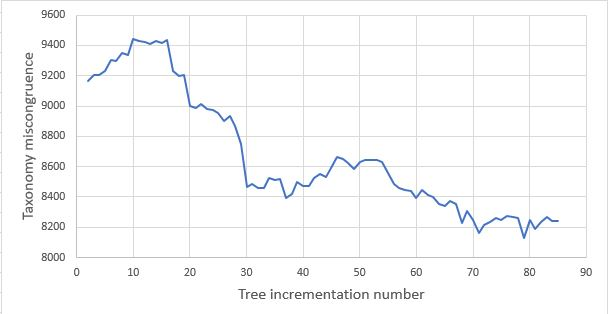
\includegraphics[scale=0.7]{ITS_Iter_TaxMisc.jpg}
  \caption{Improvement of the taxonomy miscongruence of the initial set of objects with the tree incrementation number in the Fungal ITS tree~\cite{inc_ls_dist_tree}.}
  \label{fig:Incr_TaxMisc}
\end{figure}

This suggests the following method to improve a phylogenetic tree for a set~$S$ of objects:
\begin{itemize}
  \item add more objects to~$S$ making a superset~$S'$: $S \subset S'$;
  \item build a tree for the superset~$S'$;
  \item remove the extra objects $S' \setminus S$ from the tree.
\end{itemize}
The resulting tree will contain the original set~$S$ of objects and will be on the average better than a tree built only from~$S$.



\subsection{Bacterial type strains with probably misassigned sequence}

Type strain sequences are used as golden standard for taxonomic assignment of other sequences,
but the whether the type strain sequences themselves are correct or their taxonomic lineages are correct remains a problem.

The bacterial genomes of type strains with taxonomic miscongruence $\tau \ge 32$ in the tree {\tt bacteria-R12t}~\cite{inc_ls_dist_tree}
have been manually checked,
and~53 genomes which probably have been assigned to a type strain in error or where the taxonomic lineage of the type strain is incorrect
are in Table~\ref{tab:typeStrainAsm}.
% Peptococcaceae: 2 clades
% Syntrophobacterales/Desulfobacterales: mixed
% Synechococcaceae: mixed
% Sinorhizobium/Ensifer: mixed
% Thermoanaerobacteraceae: scattered

The same manual analysis has been done for prokaryotic type strain 16S rRNA sequences using the tree {\tt prok-16S-R4}~\cite{inc_ls_dist_tree},
and~68 16S rRNA sequences which probably have been assigned to a type strain in error or where the taxonomic lineage of the type strain is incorrect,
are in Table~\ref{tab:typeStrain16S}.


\begin{table}
  \small
  \centering
  \scalebox{0.8} 
  {
  \begin{tabular}{|c|c|c|l|l|}
    \hline
   NCBI assembly & Strain &	$\tau$ &	Taxonomic lineage &	Phylogenetic lineage \\
    \hline
GCA\_900167375.1	&	ATCC 25662	&	200	&	Anaerorhabdus furcosa; Anaerorhabdus; Ba...	&	Erysipelotrichaceae; Clostridia; Terraba...	\\
GCA\_002934545.1	&	DSM 3808	&	198	&	Bacteroides xylanolyticus; Bacteroides \textless ...	&	Lachnoclostridium; Lachnospiraceae; Clos...	\\
GCA\_003847445.2	&	X0209	&	194	&	Kroppenstedtia sanguinis; Kroppenstedtia...	&	Gordoniaceae/Gordonia \textless actinomycete\textgreater ; Co...	\\
GCA\_900169515.1	&	Marseille-P3369	&	183	&	Varibaculum timonense; Varibaculum; Acti...	&	Tissierellaceae; Tissierellia; Clostridi...	\\
GCA\_006740705.1	&	NKC3-5	&	172	&	Salicibibacter halophilus; Salicibibacte...	&	Bacillaceae; ; Bacillales; Bacilli; Clos...	\\
GCA\_003051055.1	&	DSM 5822	&	166	&	Agitococcus lubricus; Agitococcus; Carno...	&	Thiotrichales; ; Gammaproteobacteria; Pr...	\\
GCA\_002362315.1	&	ATCC 31363	&	148	&	Pseudomonas acidophila; Pseudomonas; Pse...	&	Paraburkholderia; Burkholderiaceae; Burk...	\\
GCA\_002894665.1	&	CB7	&	138	&	Salinivenus iranica; Salinivenus; Salini...	&	Bacteroidetes \textless phylum\textgreater /Rhodothermaceae; ...	\\
GCA\_900114705.1	&	ATCC 43154	&	126	&	Rugamonas rubra; Rugamonas; Pseudomonada...	&	Oxalobacteraceae; Burkholderiales; Betap...	\\
GCA\_900290205.1	&	Marseille-P4302	&	126	&	Anaerolactibacter massiliensis; Anaerola...	&	Erysipelotrichaceae; Clostridia; Terraba...	\\
GCA\_003254275.1	&	DSM 6779	&	103	&	Cytophaga xylanolytica; Cytophaga; Cytop...	&	Bacteroidia/Bacteroidales; Bacteroidetes...	\\
GCA\_007970665.1	&	BR7-21	&	100	&	Baekduia soli; Baekduia; Baekduiaceae; R...	&	Solirubrobacterales; Thermoleophilia; Ac...	\\
GCA\_000483165.1	&	ATCC 49900	&	90	&	Acholeplasma multilocale ATCC 49900; Ach...	&	Mesoplasma; Entomoplasmataceae; Entomopl...	\\
GCA\_000717315.1	&	NRRL B-24431	&	90	&	Actinospica acidiphila; Actinospica; Act...	&	Streptomycetales/Streptomyces; Actinobac...	\\
GCA\_002529455.1	&	TRM 49117	&	90	&	Glycomyces fuscus; Glycomyces; Glycomyce...	&	Nocardiopsis; Nocardiopsaceae; Streptosp...	\\
GCA\_003052455.1	&	ATCC 31213	&	90	&	Sphaerisporangium cinnabarinum; Sphaeris...	&	Promicromonosporaceae/Cellulosimicrobium...	\\
GCA\_000473895.1	&	KORDI 51-2	&	76	&	Rubidibacter lacunae KORDI 51-2; Rubidib...	&	Synechococcales; ; Cyanobacteria/Melaina...	\\
GCA\_000382325.1	&	DSM 17123	&	68	&	Woodsholea maritima DSM 17123; Woodshole...	&	Rhodobacterales/Hyphomonadaceae; Alphapr...	\\
GCA\_000688235.1	&	DSM 6293	&	68	&	Terasakiella pusilla DSM 6293; Terasakie...	&	Rhodospirillaceae; Rhodospirillales; Alp...	\\
GCA\_003725335.1	&	DSM 22242	&	68	&	Parvibacter caecicola; Parvibacter; Cori...	&	Eggerthellales/Eggerthellaceae; Coriobac...	\\
GCA\_900100455.1	&	930I	&	68	&	Roseospirillum parvum; Roseospirillum; R...	&	Rhodospirillaceae; Rhodospirillales; Alp...	\\
GCA\_003574215.1	&	TH-1	&	63	&	Hydrogenophilus thermoluteolus; Hydrogen...	&	Proteobacteria; Bacteria \textless prokaryotes\textgreater ...	\\
GCA\_001855385.1	&	DSM 1989	&	62	&	Andreesenia angusta; Andreesenia; Gottsc...	&	Tissierellia; Clostridiales; Clostridia;...	\\
GCA\_001274725.1	&	DSM 4	&	48	&	Sporosarcina globispora; Sporosarcina; P...	&	Bacillus \textless bacterium\textgreater ; Bacillaceae; ; Bac...	\\
GCA\_900626075.1	&	Marseille-P8228	&	48	&	Clostridium transplantifaecale; Clostrid...	&	Lachnoclostridium; Lachnospiraceae; Clos...	\\
GCA\_900102225.1	&	i6	&	44	&	Eubacterium pyruvativorans; Eubacterium;...	&	Clostridiales; Clostridia; Terrabacteria...	\\
GCA\_001443605.1	&	L21-Spi-D4	&	42	&	Salinivirga cyanobacteriivorans; Saliniv...	&	Bacteroidia/Bacteroidales; Bacteroidetes...	\\
GCA\_000155205.1	&	ATCC 29176	&	37	&	Ruminococcus lactaris ATCC 29176; Rumino...	&	Lachnospiraceae; Clostridiales; Clostrid...	\\
GCA\_000518685.1	&	ATCC 35991	&	37	&	Eubacterium xylanophilum ATCC 35991; Eub...	&	Lachnospiraceae; Clostridiales; Clostrid...	\\
GCA\_900167085.1	&	ATCC 17233	&	37	&	Eubacterium ruminantium; Eubacterium; Eu...	&	Lachnospiraceae; Clostridiales; Clostrid...	\\
GCA\_900167205.1	&	ATCC 51222	&	37	&	Eubacterium coprostanoligenes; Eubacteri...	&	Ruminococcaceae; Clostridiales; Clostrid...	\\
GCA\_000174415.1	&	AHT 1	&	34	&	Dethiobacter alkaliphilus AHT 1; Dethiob...	&	Clostridia; Terrabacteria group/Firmicut...	\\
GCA\_000374145.1	&	DSM 15528	&	34	&	Neomegalonema perideroedes DSM 15528; Ne...	&	Alphaproteobacteria; Proteobacteria; Bac...	\\
GCA\_000384415.1	&	PS-1	&	34	&	Cycloclasticus pugetii PS-1; Cycloclasti...	&	Gammaproteobacteria; Proteobacteria; Bac...	\\
GCA\_000422285.1	&	DSM 4660	&	34	&	Desulfatiglans anilini DSM 4660; Desulfa...	&	Proteobacteria/Deltaproteobacteria; Bact...	\\
GCA\_000620305.1	&	DSM 16504	&	34	&	Desulfitibacter alkalitolerans DSM 16504...	&	Clostridiales; Clostridia; Terrabacteria...	\\
GCA\_002088235.1	&	22II-S10r2	&	34	&	Oceanococcus atlanticus; Oceanococcus; E...	&	Gammaproteobacteria; Proteobacteria; Bac...	\\
GCA\_003148465.1	&	DSM 24906	&	34	&	Oceanotoga teriensis; Oceanotoga; Thermo...	&	Thermotogae \textless phylum\textgreater /Thermotogae \textless 	\\
GCA\_003751635.1	&	DSM 100275	&	34	&	Inmirania thermothiophila; Inmirania; Ec...	&	Gammaproteobacteria; Proteobacteria; Bac...	\\
GCA\_009602465.1	&	2-36	&	34	&	Cumulibacter manganitolerans; Cumulibact...	&	Actinobacteria \textless class\textgreater ; Actinobacteria 	\\
GCA\_900086705.1	&	Marseille-P2411	&	34	&	Massilibacillus massiliensis; Massilibac...	&	Negativicutes; Terrabacteria group/Firmi...	\\
GCA\_900101835.1	&	DSM 20475	&	34	&	Peptococcus niger; Peptococcus; Peptococ...	&	Clostridia; Terrabacteria group/Firmicut...	\\
GCA\_900129455.1	&	DSM 45627	&	34	&	Jatrophihabitans endophyticus; Jatrophih...	&	Actinobacteria \textless class\textgreater ; Actinobacteria 	\\
GCA\_004362405.1	&	DSM 25082	&	33	&	Kinneretia asaccharophila; Kinneretia; C...	&	Burkholderiales; Betaproteobacteria; Pro...	\\
GCA\_004362975.1	&	DSM 28287	&	33	&	Aminicella lysinilytica; Aminicella; Eub...	&	Clostridiales; Clostridia; Terrabacteria...	\\
GCA\_007004765.1	&	GYP-15	&	33	&	Aliikangiella marina; Aliikangiella; Kan...	&	Oceanospirillales; Thiotrichales; ; Gamm...	\\
GCA\_900167975.1	&	DSM 25262	&	33	&	Ohtaekwangia koreensis; Ohtaekwangia; Cy...	&	Cytophagia/Cytophagales; Bacteroidetes \textless ...	\\
    \hline    
\end{tabular}
}
\caption{Bacterial type strain genomes which probably have been assigned to a type strain in error or where the taxonomic lineage of the type strain is incorrect. The data are as of January 2020.}
\label{tab:typeStrainAsm}
\end{table}



\begin{table}
  \small
  \centering
  \scalebox{0.8} 
  {
    \begin{tabular}{|c|c|c|l|l|}
      \hline
      \makecell{RefSeq \\ accession} & \makecell{GenBank \\ accession} &	$\tau$ &	Taxonomic lineage &	Phylogenetic lineage \\
      \hline
NR\_044819.1	&	X55406	&	231	&	Filifactor alocis; Filifactor; Peptostre...	&	Fusobacterium; Fusobacteriaceae; Fusobac...	\\
NR\_115176.1	&	AY230768	&	231	&	Paenibacillus sanguinis; Paenibacillus; ...	&	Lysobacter; Xanthomonadaceae; Xanthomona...	\\
NR\_104743.1	&	FR733681	&	226	&	Ilyobacter delafieldii; Ilyobacter; Fuso...	&	Clostridium; Clostridiaceae; Clostridial...	\\
NR\_104899.1	&	HF558386	&	226	&	Bacteroides xylanolyticus; Bacteroides \textless ...	&	Lachnoclostridium; Lachnospiraceae; Clos...	\\
NR\_104962.1	&	JX986959	&	226	&	Flavobacterium acidificum; Flavobacteriu...	&	Pantoea; Erwiniaceae; Enterobacterales; ...	\\
NR\_104868.1	&	HE582776	&	204	&	Agitococcus lubricus; Agitococcus; Carno...	&	Pseudomonadales/Moraxellaceae; Gammaprot...	\\
NR\_118671.1	&	L34614	&	203	&	Clostridium combesii; Clostridium; Clost...	&	Acidipropionibacterium; Propionibacteria...	\\
NR\_104948.1	&	JN175353	&	129	&	Prolinoborus fasciculus; Prolinoborus; N...	&	Acinetobacter; Pseudomonadales/Moraxella...	\\
NR\_117112.1	&	FR733683	&	129	&	Cytophaga xylanolytica; Cytophaga; Cytop...	&	Marinilabiliaceae; Marinilabiliales; Bac...	\\
NR\_041304.1	&	AB210824	&	118	&	Sharpea azabuensis; Sharpea; Lactobacill...	&	Firmicutes/Erysipelotrichaceae; Terrabac...	\\
NR\_104915.1	&	HM038005	&	118	&	Rugamonas rubra; Rugamonas; Pseudomonada...	&	Oxalobacteraceae; Burkholderiales; Betap...	\\
NR\_112167.1	&	AB073978	&	118	&	Fucophilus fucoidanolyticus; Fucophilus;...	&	Puniceicoccales/Puniceicoccaceae; Opitut...	\\
NR\_144718.1	&	LN713275	&	118	&	Beduini massiliensis; Beduini; Clostridi...	&	Firmicutes/Erysipelotrichaceae; Terrabac...	\\
NR\_104836.1	&	GU269544	&	116	&	Lactobacillus rogosae; Lactobacillus; La...	&	Lachnospiraceae; Clostridiales; Terrabac...	\\
NR\_147732.1	&	LC055729	&	105	&	Filobacterium rodentium; Filobacterium; ...	&	Chitinophagia/Chitinophagaceae; Bacteroi...	\\
NR\_113504.1	&	AB663439	&	100	&	Halostagnicola alkaliphila; Halostagnico...	&	Halosimplex carlsbadense; Halosimplex; H...	\\
NR\_041204.1	&	AB184754	&	95	&	Streptomyces gardneri; Streptomyces; Str...	&	Nocardia; Nocardiaceae; Corynebacteriale...	\\
NR\_043396.1	&	D14125	&	95	&	Halorubrum trapanicum; Halorubrum; Halor...	&	Natrinema; Natrialbales/Natrialbaceae; H...	\\
NR\_044137.1	&	EF178675	&	95	&	Actinoalloteichus cyanogriseus; Actinoal...	&	Streptomyces; Streptomycetales/Streptomy...	\\
NR\_104535.1	&	EU693576	&	95	&	Prauserella marina; Prauserella; Pseudon...	&	Streptomyces griseus group/Streptomyces ...	\\
NR\_115779.1	&	DQ442518	&	95	&	Streptomyces libani; Streptomyces; Strep...	&	Arthrobacter; Micrococcaceae; Micrococca...	\\
NR\_117484.1	&	GU269552	&	95	&	Pilimelia columellifera subsp. pallida; ...	&	Streptomyces; Streptomycetales/Streptomy...	\\
NR\_042487.1	&	AM183347	&	90	&	Rheinheimera perlucida; Rheinheimera; Ch...	&	Alteromonadales/Alishewanella; Chromatia...	\\
NR\_044657.2	&	M22351	&	88	&	Asteroleplasma anaerobium; Asteroleplasm...	&	Terrabacteria group/Clostridia; bacteria...	\\
NR\_117160.1	&	FR749963	&	82	&	Thermohydrogenium kirishiense; Thermohyd...	&	Thermoanaerobacterium; Thermoanaerobacte...	\\
NR\_042960.1	&	AY538169	&	79	&	Acholeplasma multilocale; Acholeplasma; ...	&	Entomoplasmataceae; Entomoplasmatales/Sp...	\\
NR\_112013.1	&	AB006157	&	79	&	Parvopolyspora pallida; Parvopolyspora; ...	&	Actinomadura; Thermomonosporaceae; Strep...	\\
NR\_025605.1	&	AJ578476	&	68	&	Woodsholea maritima; Woodsholea; Cauloba...	&	Hyphomonadaceae; Rhodobacterales; Rhizob...	\\
NR\_041955.1	&	AJ011919	&	68	&	Roseospirillum parvum; Roseospirillum; R...	&	Rhodospirillaceae; Rhodospirillales; Alp...	\\
NR\_116378.1	&	EU588727	&	68	&	Oceanotoga teriensis; Oceanotoga; Thermo...	&	Petrotogales/Petrotogaceae; Thermotogae ...	\\
NR\_156875.1	&	KF022043.1	&	68	&	Haloactinomyces albus; Haloactinomyces; ...	&	Pseudonocardiales/Pseudonocardiaceae; Ac...	\\
NR\_118544.1	&	KC188660	&	60	&	Keratinibaculum paraultunense; Keratinib...	&	Tissierellales; Tissierellia; Clostridia...	\\
NR\_028816.1	&	AF349724	&	59	&	Turicibacter sanguinis; Turicibacter; Er...	&	Terrabacteria group/Clostridia; bacteria...	\\
NR\_041385.1	&	AB245479	&	55	&	Sulfurivirga caldicuralii; Sulfurivirga;...	&	Chromatiales; Gammaproteobacteria; Oligo...	\\
NR\_137384.1	&	KP178167	&	55	&	Alkalimarinus sediminis; Alkalimarinus; ...	&	Oceanospirillales; Gammaproteobacteria; ...	\\
NR\_042854.1	&	AY345990	&	53	&	Entomoplasma melaleucae; Entomoplasma; E...	&	Entomoplasmatales/Spiroplasma; Tenericut...	\\
NR\_112008.1	&	AB004752	&	53	&	Serratia liquefaciens; Serratia; Yersini...	&	Klebsiella; Enterobacteriaceae; Enteroba...	\\
NR\_112014.1	&	AB006170	&	53	&	Sphaerimonospora mesophila NBRC 14179 = ...	&	Thermobifida; Nocardiopsaceae; Streptosp...	\\
NR\_119056.1	&	X74709	&	53	&	Moritella marina ATCC 15381; Moritella m...	&	Pseudoalteromonas; Pseudoalteromonadacea...	\\
NR\_104808.1	&	FR749965	&	50	&	Thermohydrogenium kirishiense; Thermohyd...	&	Thermoanaerobacterium; Thermoanaerobacte...	\\
NR\_117161.1	&	FR749964	&	50	&	Thermohydrogenium kirishiense; Thermohyd...	&	Thermoanaerobacterium; Thermoanaerobacte...	\\
NR\_024683.1	&	AB018184	&	48	&	Eubacterium multiforme; Eubacterium; Eub...	&	Clostridium; Clostridiaceae; Clostridial...	\\
NR\_028884.1	&	AJ132943	&	48	&	Microlunatus lacustris; Microlunatus; Pr...	&	Nocardioidaceae/Friedmanniella; Propioni...	\\
NR\_074975.1	&	CP000482	&	48	&	Pelobacter propionicus; Pelobacter; Desu...	&	Geobacteraceae/Geobacter; Desulfuromonad...	\\
NR\_115528.1	&	D16278	&	48	&	Bacillus racemilacticus; Bacillus \textless bacte...	&	Sporolactobacillaceae/Sporolactobacillus...	\\
NR\_104905.1	&	HM037993	&	46	&	Vitreoscilla filiformis; Vitreoscilla; N...	&	Burkholderiales; Betaproteobacteria; Gam...	\\
NR\_134756.1	&	HF947551	&	46	&	Limisphaera ngatamarikiensis; Limisphaer...	&	Verrucomicrobia; PVC group; bacteria; pr...	\\
NR\_029181.1	&	U16758	&	45	&	Mycoplasma feliminutum; Mycoplasma; Myco...	&	Tenericutes/Mollicutes; Terrabacteria gr...	\\
NR\_113170.1	&	AB558581	&	43	&	Oligosphaera ethanolica; Oligosphaera; O...	&	bacteria; prokaryotes...	\\
NR\_137400.1	&	JF304644	&	43	&	Chitinispirillum alkaliphilum; Chitinisp...	&	bacteria; prokaryotes...	\\
NR\_149251.1	&	LN833202	&	43	&	Longimicrobium terrae; Longimicrobium; L...	&	bacteria; prokaryotes...	\\
NR\_040915.1	&	AB078062	&	42	&	Hugenholtzia roseola; Hugenholtzia; Bern...	&	Microscillaceae; Cytophagia/Cytophagales...	\\
NR\_111998.1	&	AB004691	&	42	&	Pantoea agglomerans; Pantoea agglomerans...	&	Enterobacteriaceae; Enterobacterales; Ga...	\\
NR\_152675.1	&	LM999900	&	42	&	Balneicella halophila; Balneicella; Baln...	&	Marinilabiliales; Bacteroidia; Bacteroid...	\\
NR\_041036.1	&	AB175654	&	40	&	Azomonas macrocytogenes; Azomonas; Azoto...	&	Pseudomonas; Pseudomonadales/Pseudomonad...	\\
NR\_024661.1	&	AB008552	&	37	&	Eubacterium ruminantium; Eubacterium; Eu...	&	Lachnospiraceae; Clostridiales; Terrabac...	\\
NR\_027579.1	&	L76602	&	37	&	Ruminococcus lactaris ATCC 29176; Rumino...	&	Lachnospiraceae; Clostridiales; Terrabac...	\\
NR\_104737.1	&	FR733672	&	37	&	Eubacterium oxidoreducens; Eubacterium; ...	&	Lachnospiraceae; Clostridiales; Terrabac...	\\
NR\_104931.1	&	JN175336	&	37	&	Carbophilus carboxidus; Carbophilus; Rhi...	&	Aminobacter; Mesorhizobium; Phyllobacter...	\\
NR\_115118.1	&	AY026916	&	37	&	Lutibacterium anuloederans; Lutibacteriu...	&	Erythrobacter; Altererythrobacter; Eryth...	\\
NR\_116306.1	&	EU401907	&	37	&	Beijerinckia fluminensis; Beijerinckia; ...	&	Rhizobium/Agrobacterium group/Rhizobium;...	\\
NR\_116747.1	&	FJ611794	&	37	&	Ruminococcus faecis JCM 15917; Ruminococ...	&	Lachnospiraceae; Clostridiales; Terrabac...	\\
NR\_118670.1	&	L34421	&	37	&	Eubacterium ventriosum; Eubacterium; Eub...	&	Lachnospiraceae; Clostridiales; Terrabac...	\\
NR\_118674.1	&	L34623	&	37	&	Eubacterium ramulus ATCC 29099; Eubacter...	&	Lachnospiraceae; Clostridiales; Terrabac...	\\
NR\_118676.1	&	L34628	&	37	&	Eubacterium xylanophilum; Eubacterium; E...	&	Lachnospiraceae; Clostridiales; Terrabac...	\\
NR\_134741.1	&	KJ023821	&	37	&	Hafnia psychrotolerans; Hafnia; Hafniace...	&	Yersiniaceae; Enterobacterales; Gammapro...	\\
NR\_135890.1	&	KF982858	&	35	&	Aestuariicella hydrocarbonica; Aestuarii...	&	Cellvibrionaceae; Cellvibrionales; Gamma...	\\
NR\_159172.1	&	LN651200.1	&	35	&	Gellertiella hungarica; Gellertiella; Rh...	&	Rhizobium/Agrobacterium group/Rhizobium;...	\\
    \hline    
\end{tabular}
}
\caption{Bacterial type strain 16S rRNA sequences which probably have been assigned to a type strain in error or where the taxonomic lineage of the type strain is incorrect.
  The data are as of June 2019.}
\label{tab:typeStrain16S}
\end{table}




\subsection{Analysis of the MLST clades of {\it Escherichia coli}}

For the GenBank genomes assigned to {\it Escherichia coli} the 7-locus ST numbers have been identified using the data from \url{http://enterobase.warwick.ac.uk/species/ecoli/download_data}.
And the obtained ST numbers have been used as taxonomy extension and assigned to the interior nodes of the phylogenetic tree of GenBank bacterial genomes~\cite{inc_ls_dist_tree}
by the method described in Section~\ref{sec:assignName}.

Some ST numbers are polyphyletic,
and some ST numbers are paraphyletic, in other words, their clades contain other ST numbers.
The ST numbers with more than~50 genomes are in Table~\ref{tab:MLST}.

\begin{table}[H]
  \small
  \centering
  \scalebox{0.8} {
  \begin{tabular}{|l|r|r|r|l|}
    \hline
ST number	&	\makecell {Number of \\ genomes}&	\makecell {Number of \\genomes in \\ main clade}&	\makecell {Number \\ of clades}	&	\makecell{Clades of other ST numbers in the main clade \\	(with numbers of genomes in parentheses, $\ge 10$)}\\
    \hline
ST10	&	2062	&	1811	&	20	&	  \makecell[l]{ST34(17) ST34(96) ST43(42) ST44(15) \\
                                      ST167(149) ST227(22) ST378(13) ST617(105) \\
                                      ST744(83) ST1060(11) ST1091(13) ST1284(15)}	\\
ST11	&	1594	&	1594	&	1	&		\\
ST12	&	171	&	171	&	1	&		\\
ST14	&	91	&	91	&	1	&	ST1193(71)	\\
ST16	&	220	&	211	&	2	&	ST1792(13)	\\
ST17	&	313	&	313	&	1	&	ST1967(37)	\\
ST20	&	86	&	46	&	3	&		\\
ST21	&	785	&	785	&	1	&	ST723(23)	\\
ST23	&	344	&	339	&	4	&	ST410(233)	\\
ST29	&	1031	&	1021	&	4	&	ST21(785) ST723(23) ST765(15)	\\
ST32	&	270	&	270	&	1	&		\\
ST33	&	76	&	76	&	1	&		\\
ST34	&	113	&	96	&	2	&	ST227(22) ST378(13)	\\
ST38	&	253	&	219	&	3	&		\\
ST40	&	57	&	57	&	1	&	ST200(17)	\\
ST48	&	330	&	325	&	4	&	ST4(36) ST1312(25) ST2353(17) ST5276(17)	\\
ST58	&	97	&	95	&	2	&		\\
ST59	&	50	&	45	&	4	&		\\
ST69	&	394	&	394	&	1	&		\\
ST73	&	399	&	399	&	1	&		\\
ST88	&	157	&	87	&	4	&	ST90(26)	\\
ST93	&	166	&	100	&	4	&		\\
ST95	&	462	&	438	&	3	&	ST421(14)	\\
ST101	&	267	&	267	&	1	&	ST359(33)	\\
ST117	&	213	&	211	&	2	&	ST5935(14)	\\
ST127	&	118	&	118	&	1	&		\\
ST137	&	287	&	287	&	1	&	ST32(270)	\\
ST141	&	57	&	35	&	2	&		\\
ST154	&	55	&	51	&	2	&		\\
ST155	&	170	&	79	&	3	&		\\
ST156	&	126	&	126	&	1	&	ST348(14)	\\
ST162	&	70	&	26	&	6	&		\\
ST165	&	248	&	244	&	3	&	ST100(22) ST189(59) ST301(85)	\\
ST167	&	155	&	149	&	4	&		\\
ST173	&	81	&	81	&	1	&	ST5305(28)	\\
ST189	&	59	&	59	&	1	&		\\
ST206	&	115	&	114	&	2	&		\\
ST224	&	107	&	59	&	2	&		\\
ST245	&	68	&	62	&	2	&		\\
ST278	&	117	&	98	&	3	&	ST328(46)	\\
ST297	&	63	&	63	&	1	&		\\
ST301	&	85	&	85	&	1	&		\\
ST342	&	88	&	88	&	1	&		\\
ST349	&	56	&	56	&	1	&		\\
ST354	&	57	&	57	&	1	&		\\
ST357	&	58	&	58	&	1	&		\\
ST398	&	59	&	56	&	2	&		\\
ST399	&	69	&	69	&	1	&	ST635(29)	\\
ST405	&	181	&	164	&	4	&		\\
ST410	&	240	&	233	&	3	&		\\
ST442	&	109	&	105	&	3	&		\\
ST443	&	122	&	115	&	2	&		\\
ST448	&	54	&	54	&	1	&	ST94(15)	\\
ST453	&	61	&	61	&	1	&		\\
ST457	&	76	&	76	&	1	&		\\
ST517	&	71	&	71	&	1	&		\\
ST542	&	60	&	49	&	2	&		\\
ST602	&	73	&	73	&	1	&		\\
ST617	&	105	&	105	&	1	&	ST1284(15)	\\
ST641	&	180	&	180	&	1	&	ST86(11) ST453(61) ST877(10)	\\
ST648	&	136	&	122	&	4	&		\\
ST655	&	163	&	153	&	2	&		\\
ST678	&	91	&	91	&	1	&		\\
ST744	&	85	&	83	&	3	&		\\
ST746	&	97	&	97	&	1	&		\\
ST1193	&	71	&	71	&	1	&		\\
ST2332	&	101	&	101	&	1	&		\\
    \hline
  \end{tabular}
}
  \caption{The {\it Escherichia coli} 7-locus MLST numbers with more than 50 genomes.}
  \label{tab:MLST}
\end{table}



\section*{Acknowledgements}
I thank Richa Agarwala, Josh Cherry, Barbara Robbertse, Conrad Schoch, Bill Klimke and David Lipman for the discussions of this project.


\section*{Funding}
This research was supported by the National Center for Biotechnology Information of the National Library of Medicine (NLM), National Institutes of Health.


\section*{Availability of data and materials}
The source code for the algorithms described in this paper 
is written in C++ and {\tt bash} scripts for UNIX
and is available at \url{https://github.com/ncbi/tree-tool}.

License: Freely available to the public for use.

The documentation for this code is available at \url{https://github.com/ncbi/tree-tool/wiki}.


\section*{Authors contributions}
Not applicable.


\section*{Competing interest}
Authors declare that they have no competing interests.


\section*{Consent for publication}
Not applicable.


\section*{Ethics approval and consent to participate}
Not applicable.



\clearpage
\appendix
\appendixpage
\addappheadtotoc

\section{Encoding of taxonomical lineage for maximum parsimony problem}
\label{app:lineage}

The NCBI taxonomy as of 01/09/2020 is used.
There are 30~ranks in the NCBI taxonomy.
The {\em subranks} are taxons between ranks.
See Table~\ref{tab:rank}.

\begin{table}[h]
  \small
  \centering
  \begin{tabular}{|l|c|c|}
    \hline
    Rank name&Rank number&Max. number of subranks\\
    \hline
superkingdom	&	0	&	5	\\
kingdom	&	1	&	5	\\
subkingdom	&	2	&	1	\\
superphylum	&	3	&	0	\\
phylum	&	4	&	3	\\
subphylum	&	5	&	6	\\
superclass	&	6	&	11	\\
class	&	7	&	7	\\
subclass	&	8	&	3	\\
infraclass	&	9	&	3	\\
cohort	&	10	&	8	\\
subcohort	&	11	&	1	\\
superorder	&	12	&	1	\\
order	&	13	&	6	\\
suborder	&	14	&	3	\\
infraorder	&	15	&	4	\\
parvorder	&	16	&	2	\\
superfamily	&	17	&	1	\\
family	&	18	&	3	\\
subfamily	&	19	&	4	\\
tribe	&	20	&	1	\\
subtribe	&	21	&	1	\\
genus	&	22	&	3	\\
subgenus	&	23	&	2	\\
species group	&	24	&	1	\\
species subgroup	&	25	&	1	\\
species	&	26	&	4	\\
subspecies	&	27	&	2	\\
varietas	&	28	&	1	\\
forma	&	29	&	0	\\    \hline
\end{tabular}
\caption{Ranks in the NCBI taxonomy}
\label{tab:rank}
\end{table}

The greatest number of subranks between two consecutive ranks is~11 for rank ``superclass'',
see Table~\ref{tab:subrank}.

\begin{table}[h]
  \small
  \centering
  \begin{tabular}{|l|l|c|c|c|}
    \hline
    NCBI taxon id&Taxon name&Rank name&Rank number&Subrank number\\
    \hline
    8287    &{\it Sarcopterygii} &superclass       &6&0\\
    1338369 &{\it Dipnotetrapodomorpha} &-&-&1\\
    32523   &{\it Tetrapoda}       &-&-&2\\
    32524   &{\it Amniota}         &-&-&3\\
    8457    &{\it Sauropsida}      &-&-&4\\
    32561   &{\it Sauria}          &-&-&5\\
    1329799 &{\it Archelosauria}   &-&-&6\\
    8492    &{\it Archosauria}     &-&-&7\\
    436486  &{\it Dinosauria}      &-&-&8\\
    436489  &{\it Saurischia}      &-&-&9\\
    436491  &{\it Theropoda}       &-&-&10\\
    436492  &{\it Coelurosauria}   &-&-&11\\
    8782    &{\it Aves} (birds)     &class    &7&0\\
    \hline
  \end{tabular}
  \caption{Example of a taxonomic lineage with subranks: birds.}
  \label{tab:subrank}
\end{table}

A taxonomical lineage is encoded as a sequence of lines of the format:
\begin{center}
  {\tt rank\_number.subrank\_number:tax\_name}
\end{center}

If some ranks or subranks are missing in the lineage, they are represented in the encoding by borrowing the {\tt tax\_name} from the previous line.

The unknown taxons are recognized by the following keywords in their taxonomic names: 
unclassified, 
unassigned, 
unidentified, 
candidate phyla,
incertae sedis,
symbionts,
sp. (but not f.~sp.~which is forma speciales),
taxa,
taxon,
uncultured,
bacterium,
actinobacterium,
proteobacterium.

The unknown taxons are encoded by {\tt tax\_name = \_OTHER\_}.

For example, the lineage of taxid 2315236 is ``    cellular organisms; Bacteria; Proteobacteria; Betaproteobacteria; Burkholderiales; unclassified Burkholderiales; Burkholderiales Genera incertae sedis; Aquabacterium; Aquabacterium pictum''.
The lineage encoding is in Listing~\ref{lst:lineage}.

\begin{lstlisting}[float,captionpos=b,label=lst:lineage,caption={Encoded lineage for {\it Aquabacterium pictum}.},basicstyle=\tiny\ttfamily]
00-00:Bacteria <prokaryotes>
00-01:Bacteria <prokaryotes>
00-02:Bacteria <prokaryotes>
00-03:Bacteria <prokaryotes>
00-04:Bacteria <prokaryotes>
00-05:Bacteria <prokaryotes>
01-00:Bacteria <prokaryotes>
01-01:Bacteria <prokaryotes>
01-02:Bacteria <prokaryotes>
01-03:Bacteria <prokaryotes>
01-04:Bacteria <prokaryotes>
01-05:Bacteria <prokaryotes>
02-00:Bacteria <prokaryotes>
02-01:Bacteria <prokaryotes>
03-00:Bacteria <prokaryotes>
04-00:Proteobacteria
04-01:Proteobacteria
04-02:Proteobacteria
04-03:Proteobacteria
05-00:Proteobacteria
05-01:Proteobacteria
05-02:Proteobacteria
05-03:Proteobacteria
05-04:Proteobacteria
05-05:Proteobacteria
05-06:Proteobacteria
06-00:Proteobacteria
06-01:Proteobacteria
06-02:Proteobacteria
06-03:Proteobacteria
06-04:Proteobacteria
06-05:Proteobacteria
06-06:Proteobacteria
06-07:Proteobacteria
06-08:Proteobacteria
06-09:Proteobacteria
06-10:Proteobacteria
06-11:Proteobacteria
07-00:Betaproteobacteria
07-01:Betaproteobacteria
07-02:Betaproteobacteria
07-03:Betaproteobacteria
07-04:Betaproteobacteria
07-05:Betaproteobacteria
07-06:Betaproteobacteria
07-07:Betaproteobacteria
08-00:Betaproteobacteria
08-01:Betaproteobacteria
08-02:Betaproteobacteria
08-03:Betaproteobacteria
09-00:Betaproteobacteria
09-01:Betaproteobacteria
09-02:Betaproteobacteria
09-03:Betaproteobacteria
10-00:Betaproteobacteria
10-01:Betaproteobacteria
10-02:Betaproteobacteria
10-03:Betaproteobacteria
10-04:Betaproteobacteria
10-05:Betaproteobacteria
10-06:Betaproteobacteria
10-07:Betaproteobacteria
10-08:Betaproteobacteria
11-00:Betaproteobacteria
11-01:Betaproteobacteria
12-00:Betaproteobacteria
12-01:Betaproteobacteria
13-00:Burkholderiales
13-01:_OTHER_
13-02:_OTHER_
13-03:_OTHER_
13-04:_OTHER_
13-05:_OTHER_
13-06:_OTHER_
14-00:_OTHER_
14-01:_OTHER_
14-02:_OTHER_
14-03:_OTHER_
15-00:_OTHER_
15-01:_OTHER_
15-02:_OTHER_
15-03:_OTHER_
15-04:_OTHER_
16-00:_OTHER_
16-01:_OTHER_
16-02:_OTHER_
17-00:_OTHER_
17-01:_OTHER_
18-00:_OTHER_
18-01:_OTHER_
18-02:_OTHER_
18-03:_OTHER_
19-00:_OTHER_
19-01:_OTHER_
19-02:_OTHER_
19-03:_OTHER_
19-04:_OTHER_
20-00:_OTHER_
20-01:_OTHER_
21-00:_OTHER_
21-01:_OTHER_
22-00:Aquabacterium
22-01:Aquabacterium
22-02:Aquabacterium
22-03:Aquabacterium
23-00:Aquabacterium
23-01:Aquabacterium
23-02:Aquabacterium
24-00:Aquabacterium
24-01:Aquabacterium
25-00:Aquabacterium
25-01:Aquabacterium
26-00:Aquabacterium pictum
26-01:Aquabacterium pictum
26-02:Aquabacterium pictum
26-03:Aquabacterium pictum
26-04:Aquabacterium pictum
\end{lstlisting}


\clearpage
\begin{thebibliography}{9}

\bibitem{inc_ls_dist_tree}
Brover~S.,
Building Large Phylogenetic Trees in Log-Linear Time.
{\it In print.}
 
\bibitem{Taxonomy}
Federhen S. 
The NCBI Taxonomy database. 
Nucleic Acids Res. 2012 Jan;40(Database issue):D136-43. doi: 10.1093/nar/gkr1178. Epub 2011 Dec 1. 
PMID: 22139910; PMCID: PMC3245000.
 
\bibitem{Felsenstein}
Joseph Felsenstein. Inferring Phylogenies. Sunderland, MA: Sinauer Associates, 2003. 

\bibitem{GTDB}
Parks, D., Chuvochina, M., Waite, D. et al. 
A standardized bacterial taxonomy based on genome phylogeny substantially revises the tree of life. 
Nat Biotechnol 36, 996-1004 (2018) doi:10.1038/nbt.4229

\bibitem{CheckM}
Parks DH, Imelfort M, Skennerton CT, Hugenholtz P, Tyson GW. 
CheckM: assessing the quality of microbial genomes recovered from isolates, single cells, and metagenomes. 
Genome Res. 2015 Jul;25(7):1043-55. doi: 10.1101/gr.186072.114. 
Epub 2015 May 14. PMID: 25977477; PMCID: PMC4484387.

\bibitem{Silva}
Quast C, Pruesse E, Yilmaz P, Gerken J, Schweer T, Yarza P, Peplies J, Gl�ckner FO (2013) 
The SILVA ribosomal RNA gene database project: improved data processing and web-based tools. 
Nucl. Acids Res. 41 (D1): D590-D596. 

\bibitem{Rokas}
Shen XX et al.,
Tempo and Mode of Genome Evolution in the Budding Yeast Subphylum.
Cell. 2018 Nov 29;175(6):1533-1545.e20. doi: 10.1016/j.cell.2018.10.023. Epub 2018 Nov 8.

\bibitem{ASTRAL}
Zhu, Q., Mai, U., Pfeiffer, W. et al. 
Phylogenomics of 10,575 genomes reveals evolutionary proximity between domains Bacteria and Archaea. 
Nat Commun 10, 5477 (2019). 
https://doi.org/10.1038/s41467-019-13443-4

\end{thebibliography}


\bibliographystyle{unsrt}



\end{document}


